
\appendix
\section{Anhang}
\subsection{Pflichtenheft}\label{appendix:a1}\par
Basierend auf dem Lastenheft und unter Berücksichtigung der verfügbaren Ressourcen wurden die folgenden Anforderungen im Pflichtenheft festgelegt:

\begin{enumerate}
\item Plattform
\begin{itemize}
\item Das Backend wird mit Node.js implementiert.
\item Die Webkomponenten werden unter Verwendung von Vue.js entwickelt.
\item Die Webanwendung ist ausschließlich im Intranet erreichbar.
\item Die Webanwendung wird auf einem WildFly-Server betrieben, der innerhalb eines Docker-Containers läuft.
\item Git wird als System für die Versionskontrolle genutzt.
\item Gitea dient als gehostete Softwarelösung für die Versionsverwaltung der \acs{GSSD}.
\item Gradle wird für den automatisierten Build-Prozess verwendet.
\item Der Jenkins-Server ist für die Continuous Delivery (CD) zuständig.
\end{itemize}
\item Datenbank
\begin{itemize}
\item Die Datenbankanbindung erfolgt über Knex.js.
\item Daten, die älter als 6 Monate sind, werden gelöscht.
\item Die Daten werden in einer MariaDB-Datenbank gespeichert.
\item Die Repository-Klassen implementieren vorgegebene Interfaces, die die erforderlichen Methoden definieren.
\item Die Persistenzschicht wird mit Hilfe von Testcontainern getestet.
\end{itemize}
\item Benutzeroberfläche
\begin{itemize}
\item Die Benutzeroberflächen werden mit Vue.js erstellt.
\item Die Benutzeroberflächen werden unter Verwendung von Cascading Style Sheets (CSS) 3 gestaltet und sollen die Corporate Identity der \acs{GSSD} wahren.
\item Die Benutzeroberflächen sind nicht responsiv gestaltet.
\end{itemize}
\item Geschäftslogik
\begin{itemize}
\item Zur Erzeugung von Objekten wird Contexts and Dependency Injection (CDI) verwendet.
\item Das Framework JUnit 5 wird für automatisierte Tests eingesetzt.
\end{itemize}
\end{enumerate}
\clearpage

\subsection{Verwendete Ressourcen}\label{appendix:a2}\par
 Hardware
\begin{itemize}
	\item Laptop
\item Büroeigener Server – Bereitstellung der Testumgebung
\end{itemize}

Software
\begin{itemize}
\item Figma -- Programm zur Erstellung von Mockups
\item VSCode -- Code Editor
\item NodeJs -- plattformunabhängige JavaScript-Laufzeitumgebung
\item NPM – Package Manager für das Projekt
\item Yarn – Package Manager für das Projekt
\item VueJS -- JavaScript-Framework für Benutzeroberflächen
\item VSCode mit MiKTeX -- Entwicklungsumgebung für \LaTeX
\item Draw.io – Website zum Erstellen von Diagrammen
\item Lucidchart – Website zum Erstellen von Diagrammen
\item Git -- Verteilte Versionsverwaltung
\item Jenkins -- Buildserver
\item JUnit -- Framework zur Durchführung von Unit-Tests
\item MiKTeX -- Distribution des Textsatzsystems \TeX
\item Mockito -- Mocking-Framework zur Erstellung von Pseudoklassen
\item MariaDB -- Datenbanksystem
\item Github -- Projektmanagement
\item Windows 10 -- Betriebssystem
\item Internet Browser (Firefox, Chrome, IE) – Darstellung der lokalen Umgebung und Zugang
auf das Testsystem
\end{itemize}

 Personal
\begin{itemize}
\item Auszubildender -- Umsetzung des Projektes
\item Entwickler, Projektleiter – Umsetzung des Backends der Applikation und Review des Codes
\item Geschäftsführer – Beratung, Hilfe bei Fragestellungen, Kommunikation mit dem Kunden
\end{itemize}
Sonstiges
\begin{itemize}
\item Büro, Arbeitsplatz
\end{itemize}
\clearpage



\subsection{Anforderungen}\label{appendix:a4}\par
\begin{table}[h]
	\centering
	\begin{tabular}{ l l }
	\hline
	\rowcolor[HTML]{127017}
	\textbf{\color{white}Anforderung} & \textbf{\color{white}Beschreibung} \\
	\rowcolor[HTML]{e1efd9}
	\textbf{Funktional} & \\
	Diensteüberwachung & Überwachung der Dienste, die auf den Servern laufen \\
	Alarmierung & Benachrichtigung im Falle von Störungen \\
	Protokollierung & Aufzeichnung von Zustandsänderungen und Störungen \\
	Registrieren & neue Sensor registrieren \\
	\rowcolor[HTML]{e1efd9}
	\textbf{Nicht-Funktional} & \\
	Benutzerfreundlichkeit & Einfache Bedienbarkeit des Systems \\
	Zuverlässigkeit & Hohe Verfügbarkeit und Genauigkeit des Überwachungssystems \\
	\rowcolor[HTML]{e1efd9}
	\textbf{Qualität} & \\
	Skalierbarkeit & Möglichkeit zur Erweiterung des Systems \\
	Flexibilität & Anpassung an unterschiedliche Anforderungen des Kunden \\
	\rowcolor[HTML]{e1efd9}
	\textbf{Leistung} & \\
	Echtzeitüberwachung & Echtzeitüberwachung der Zustände \\
	Ressourcenschonung & Geringer Ressourcenverbrauch auf den überwachten Servern \\
	\end{tabular}
	\caption{Anforderungen an das Überwachungssystem}
\end{table}
\clearpage

\subsection{Komponent Diagram}\label{appendix:a5}\par
\begin{figure}[h]
	\centering
	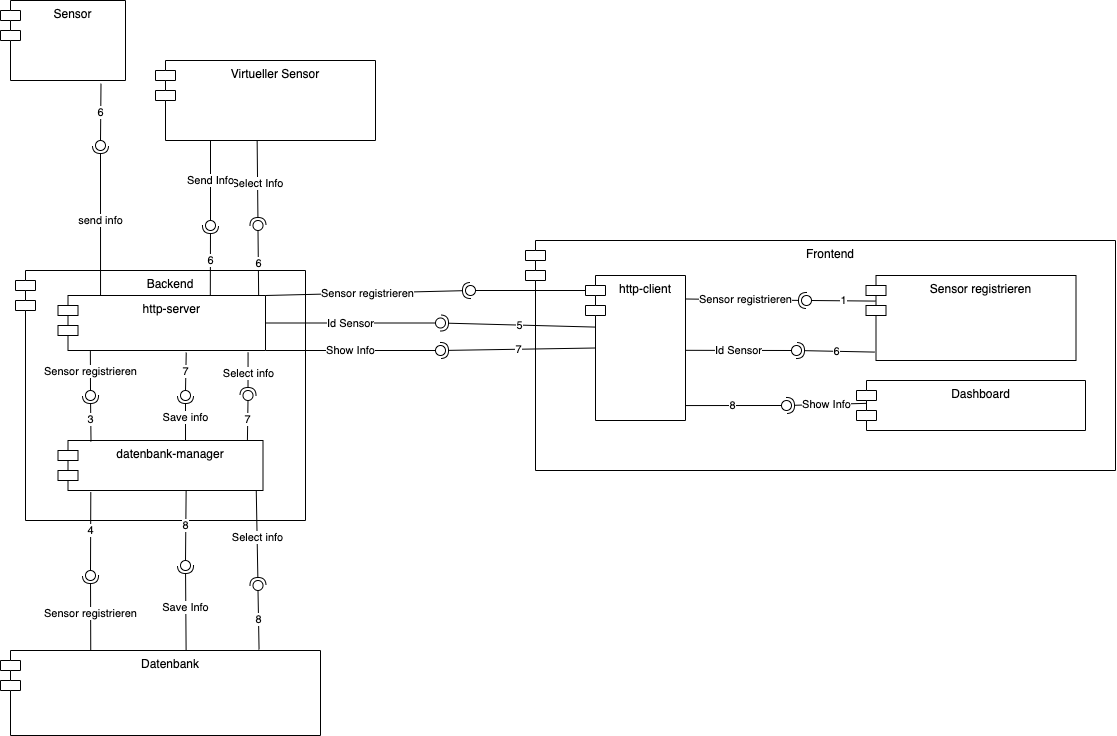
\includegraphics[width=1\textwidth]{img/komponent_diagram.png}
	\caption{Komponent Diagram}
	\label{fig:example}
\end{figure}
\clearpage

\section{Relationales Datenbankmodell}\label{appendix:a6}\par

Für dieses Projekt wurde ein Entity-Relationship-Diagramm (ER-Diagramm) erstellt, um die Struktur der Datenbank und die Beziehungen zwischen den verschiedenen Entitäten zu modellieren. Das ER-Diagramm bildet die Grundlage für das Datenbankschema und hilft bei der Organisation der Daten, die im Rahmen des Überwachungssystems erfasst und verarbeitet werden.
\begin{figure}[h]
	\centering
	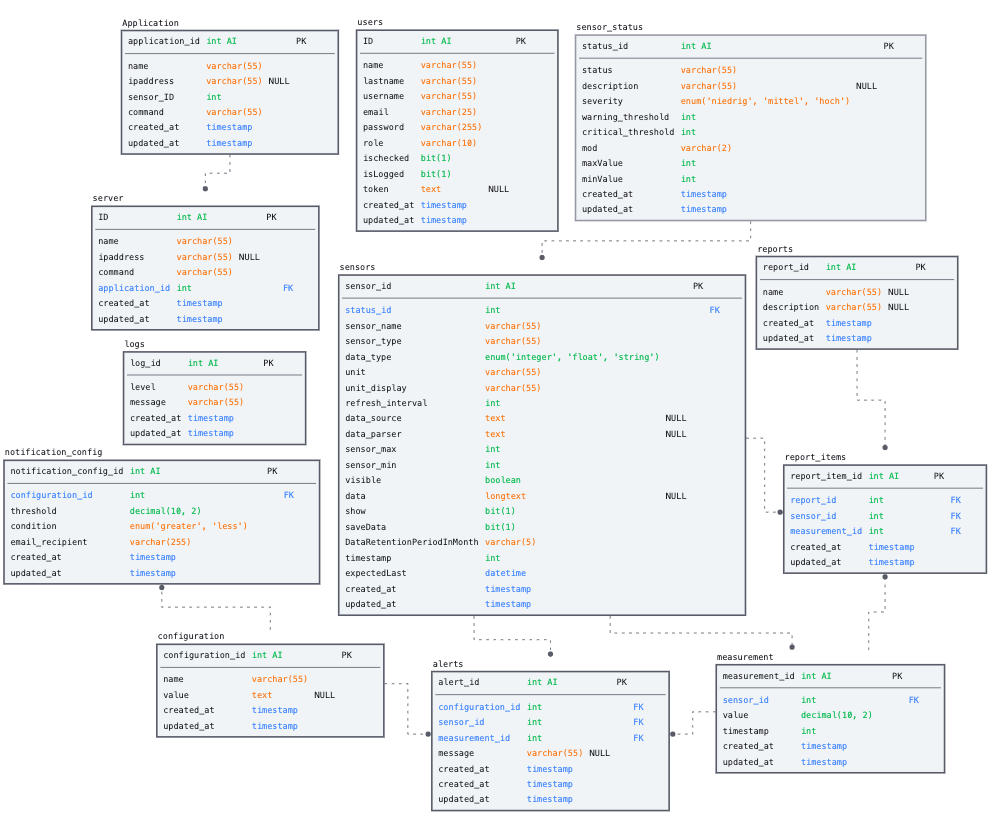
\includegraphics[width=1\textwidth]{img/ERP-diagramm.png}
	\caption{Relationales Datenbankmodell}
	\label{fig:example}
\end{figure}
\clearpage

\subsection{Screenshot des Sprint-Boards in GitHub}\label{appendix:a7}\par


In diesem Projekt wurde ein Sprint-Board in GitHub für die Planung und Verwaltung der Softwareentwicklung eingesetzt. Das Kanban Board ermöglichte eine effektive Organisation der verschiedenen Aufgaben und Phasen des Projekts, indem es den Fortschritt in Echtzeit darstellte. Als Einzelperson war das Kanban Board ein wertvolles Instrument zur Selbstorganisation und zum Nachverfolgen der Aufgaben, um sicherzustellen, dass alle notwendigen Schritte abgeschlossen und Ziele erreicht wurden.

\begin{figure}[h]
	\centering
	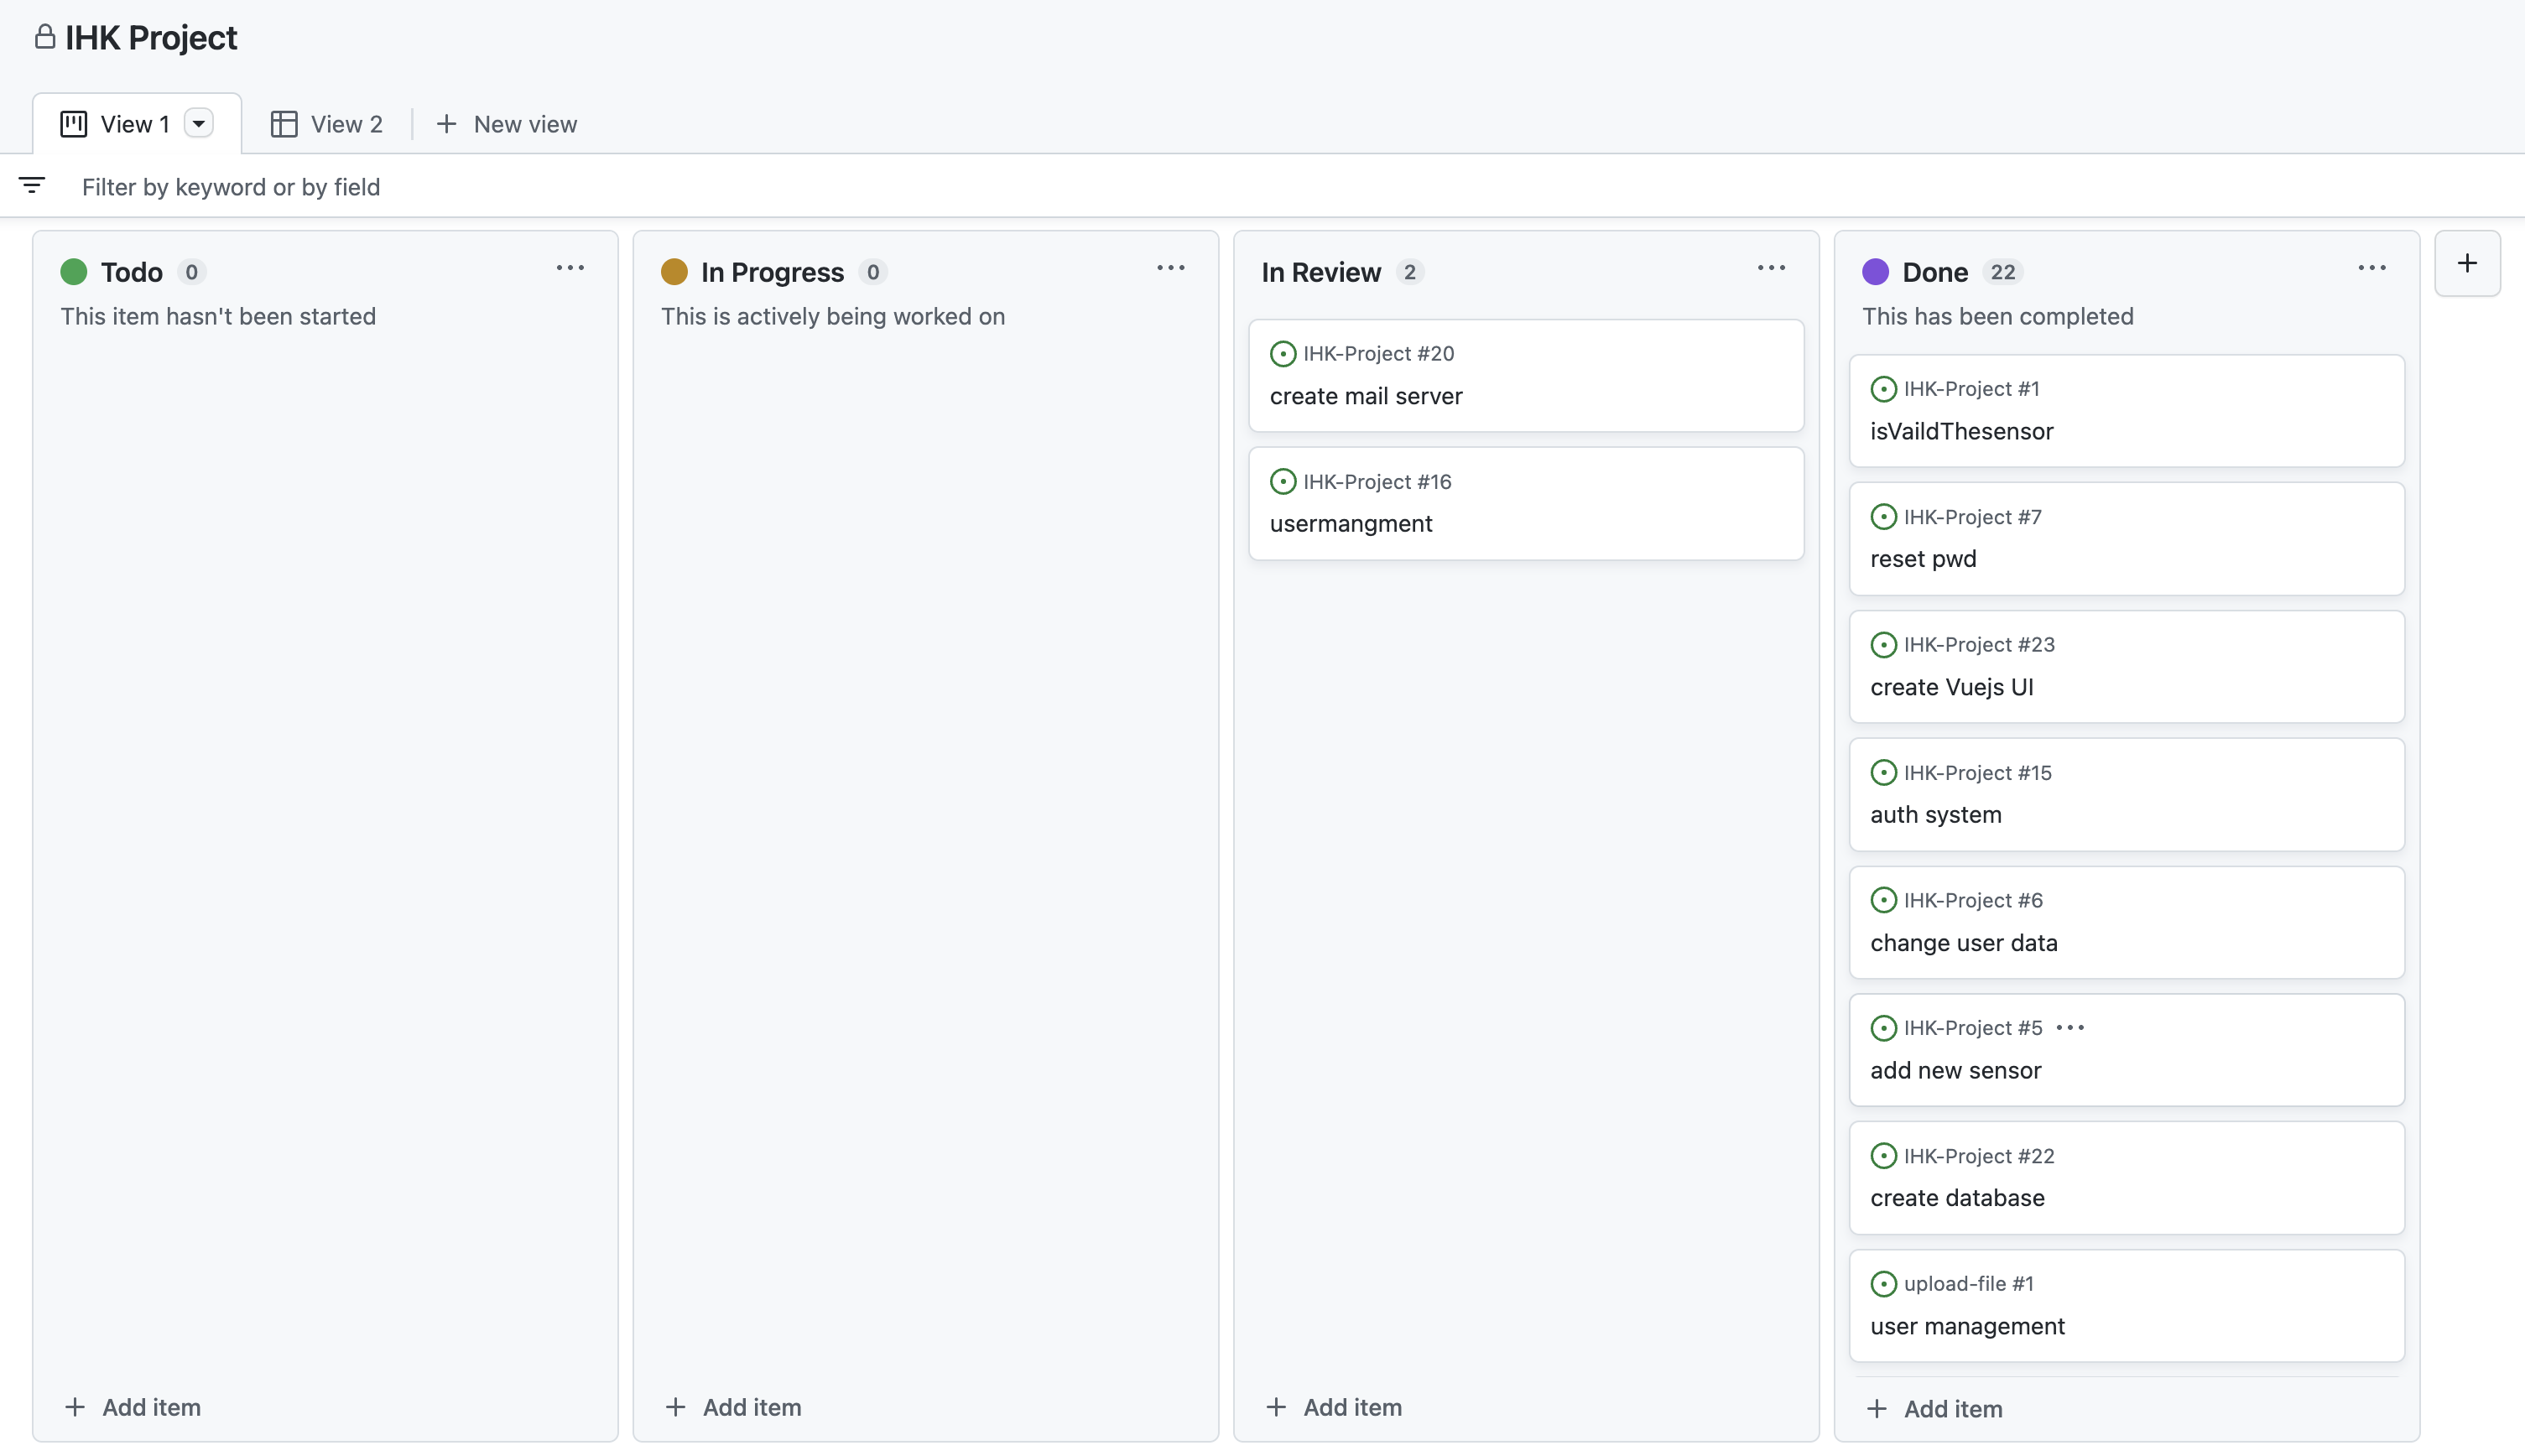
\includegraphics[width=1\textwidth]{img/github_canban.png}
	\caption{Screenshot des Sprint-Boards in GitHub}
	\label{fig:example}
\end{figure}
\clearpage

\subsection{Verwendung von Gantt-Diagramm in GitHub für die Projektplanung}\label{appendix:a8}\par

Seitdem GitHub die Unterstützung für Gantt-Diagramme in seinem Feature-Set integriert hat, ist die Planung und Verfolgung von Projekten einfacher geworden. Durch die Verwendung von Gantt-Diagrammen in GitHub können die verschiedenen Phasen des Projekts, Meilensteine und Aufgaben übersichtlich dargestellt und der Fortschritt sowie die Abhängigkeiten zwischen den einzelnen Aufgaben verfolgt werden. Dies trägt zur effektiven Planung, Zeitmanagement und zur rechtzeitigen Erreichung der Projektziele bei.
\begin{figure}[h]
	\centering
	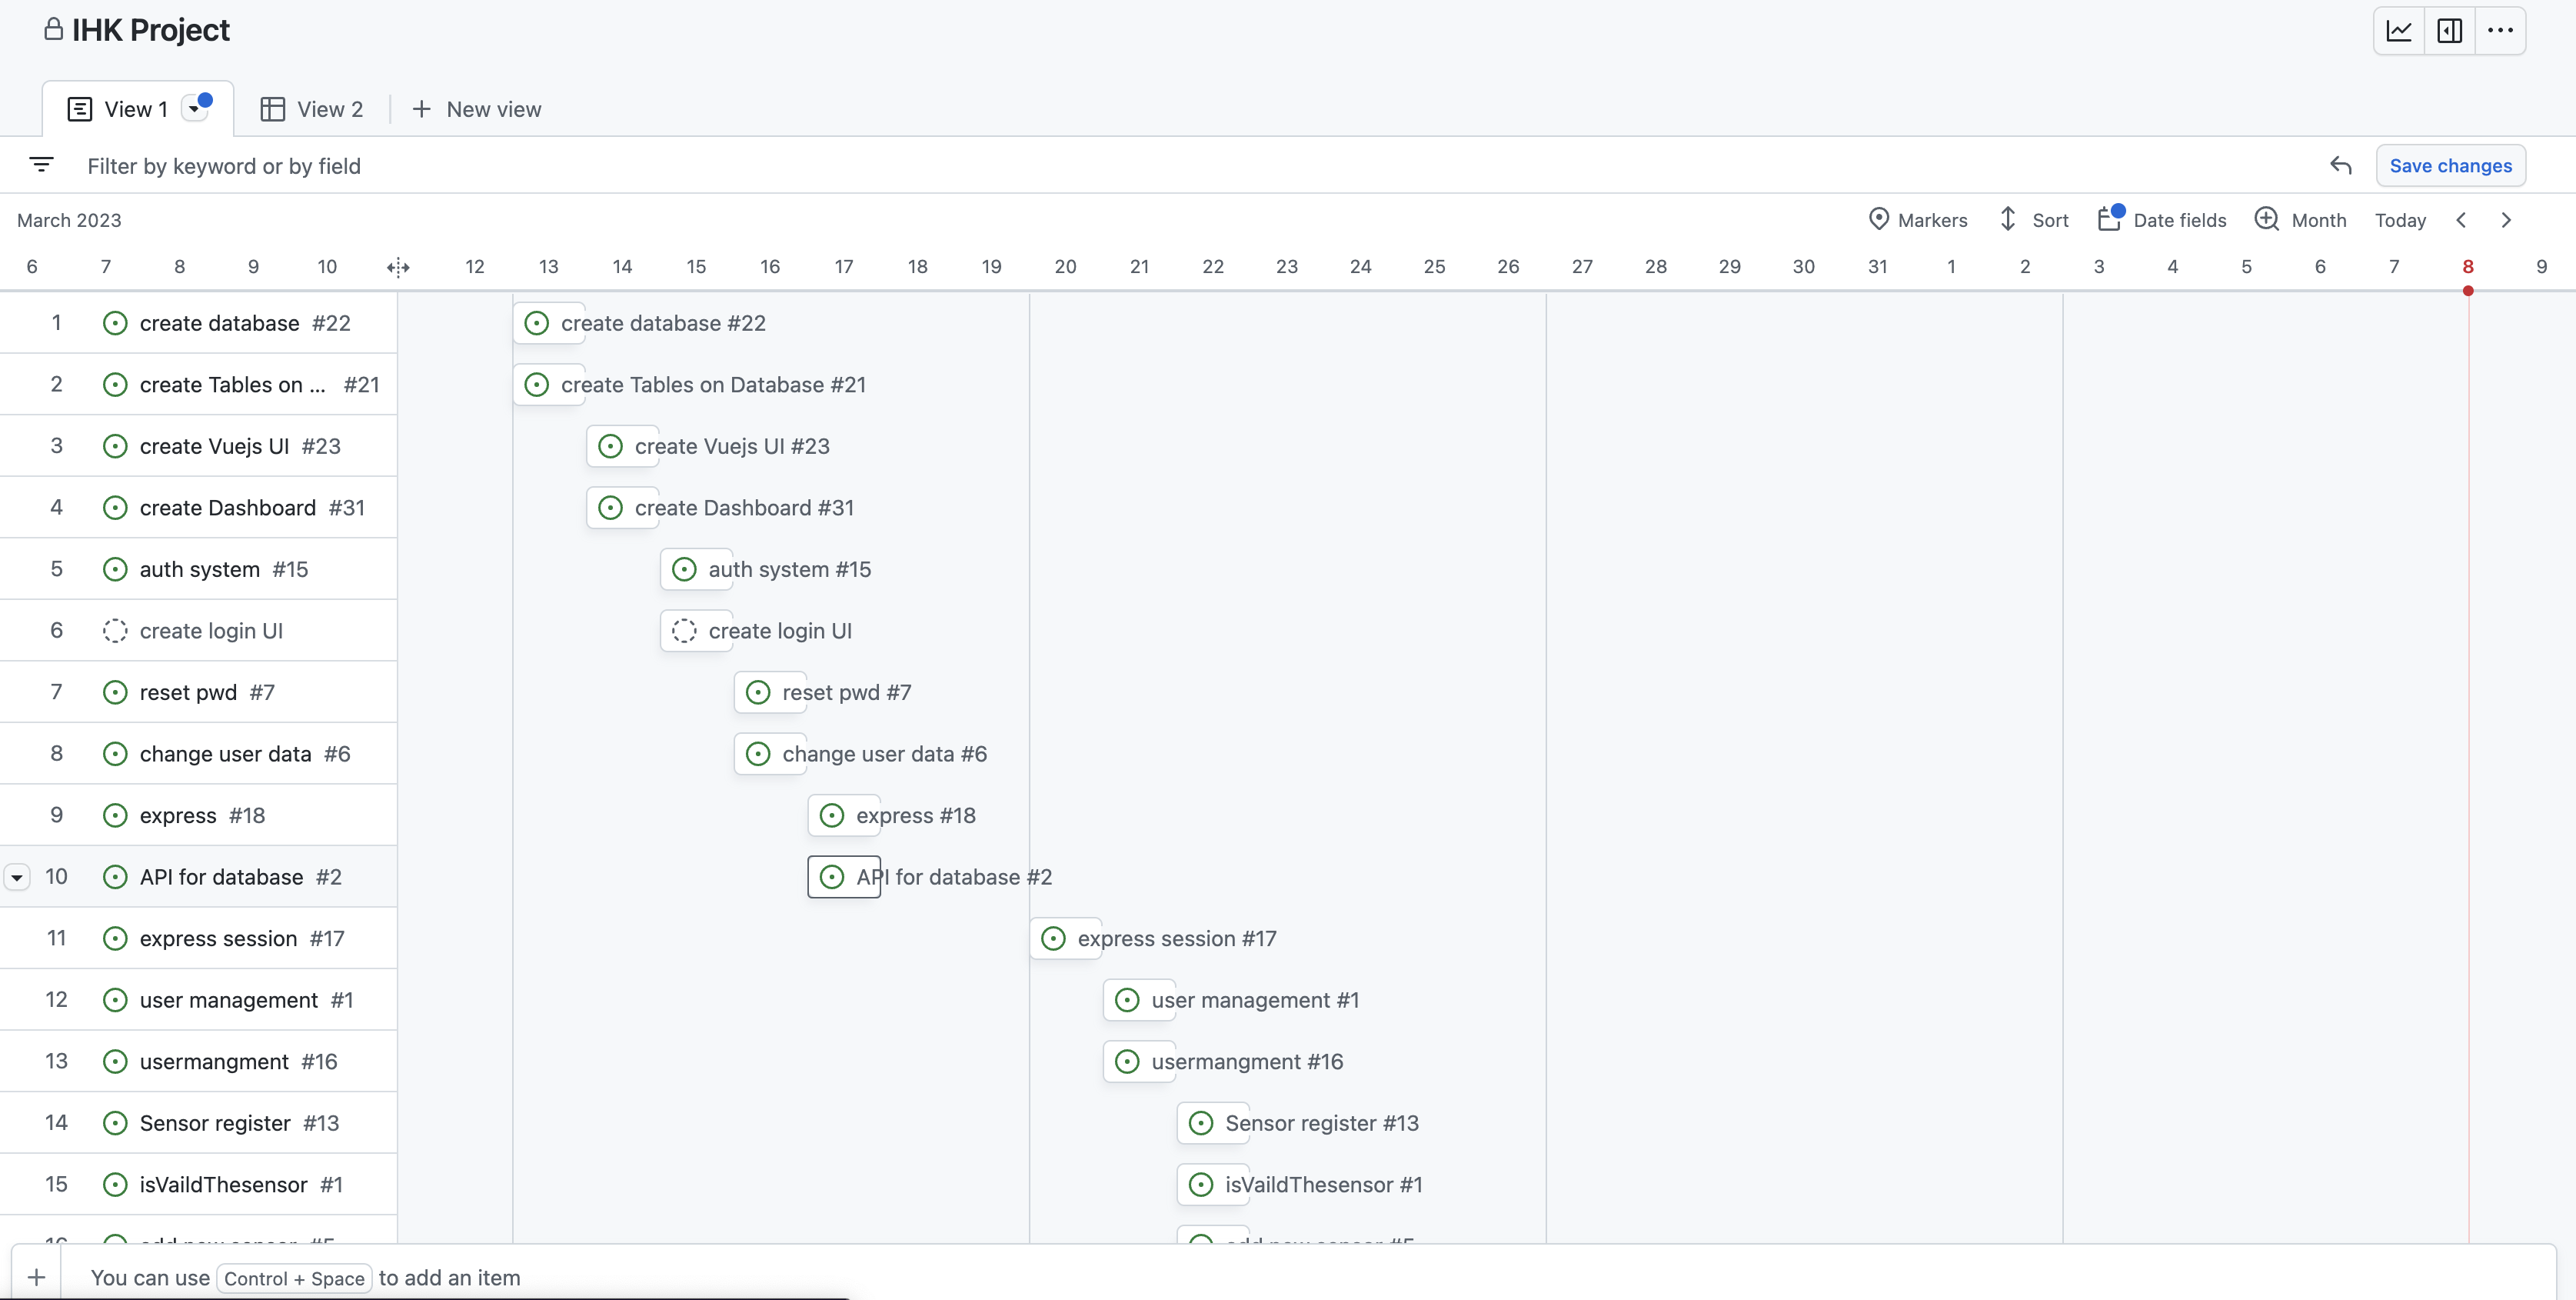
\includegraphics[width=1\textwidth]{img/github_diaramm.png}
	\caption{Verwendung von Gantt-Diagramm in GitHub für die Projektplanung}
	\label{fig:example}
\end{figure}
\clearpage


\subsection{Neue Sensor anmelden}\label{appendix:a3}\par
Im folgenden Abschnitt wird ein JavaScript-Objekt beschrieben, das einen Sensor mit dem Datentyp “integer” repräsentiert.


Mit diesem Objekt kann der Sensor seine Daten und Einstellungen an das Backend senden, um beispielsweise Daten an das Frontend zu senden oder die Daten in der Datenbank zu speichern. Das Backend verwendet diese Informationen, um den Sensor zu verwalten und seine Konfiguration zu aktualisieren.
\begin{figure}[h]
	\centering
	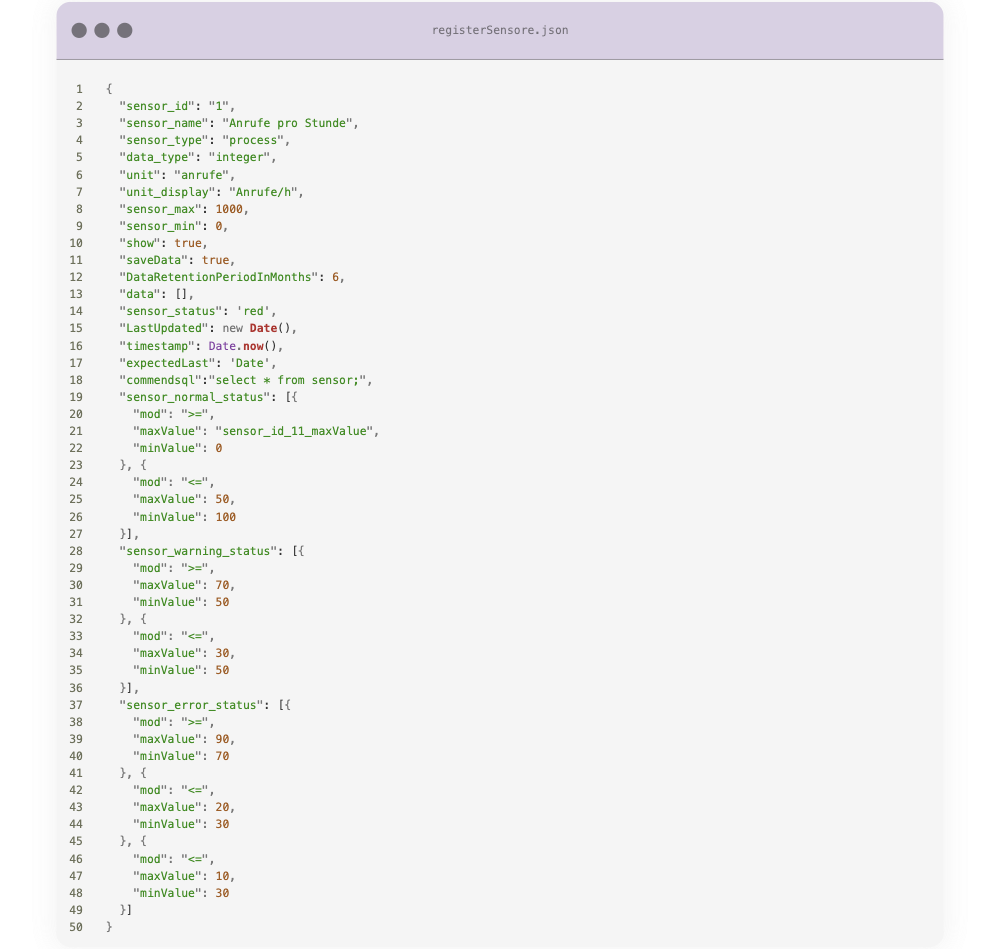
\includegraphics[width=1\textwidth]{img/registerSensore.png}
	\caption{Neue Sensor anmelden}
	\label{fig:example}
\end{figure}
\clearpage




\subsection{ein Stück Code aus Frontend}\label{appendix:a9}\par

	\clearpage

% \newpage
\subsection{Dashboard (Frontend)}\label{appendix:a6}\par
\begin{figure}[htbp]
	\centering
	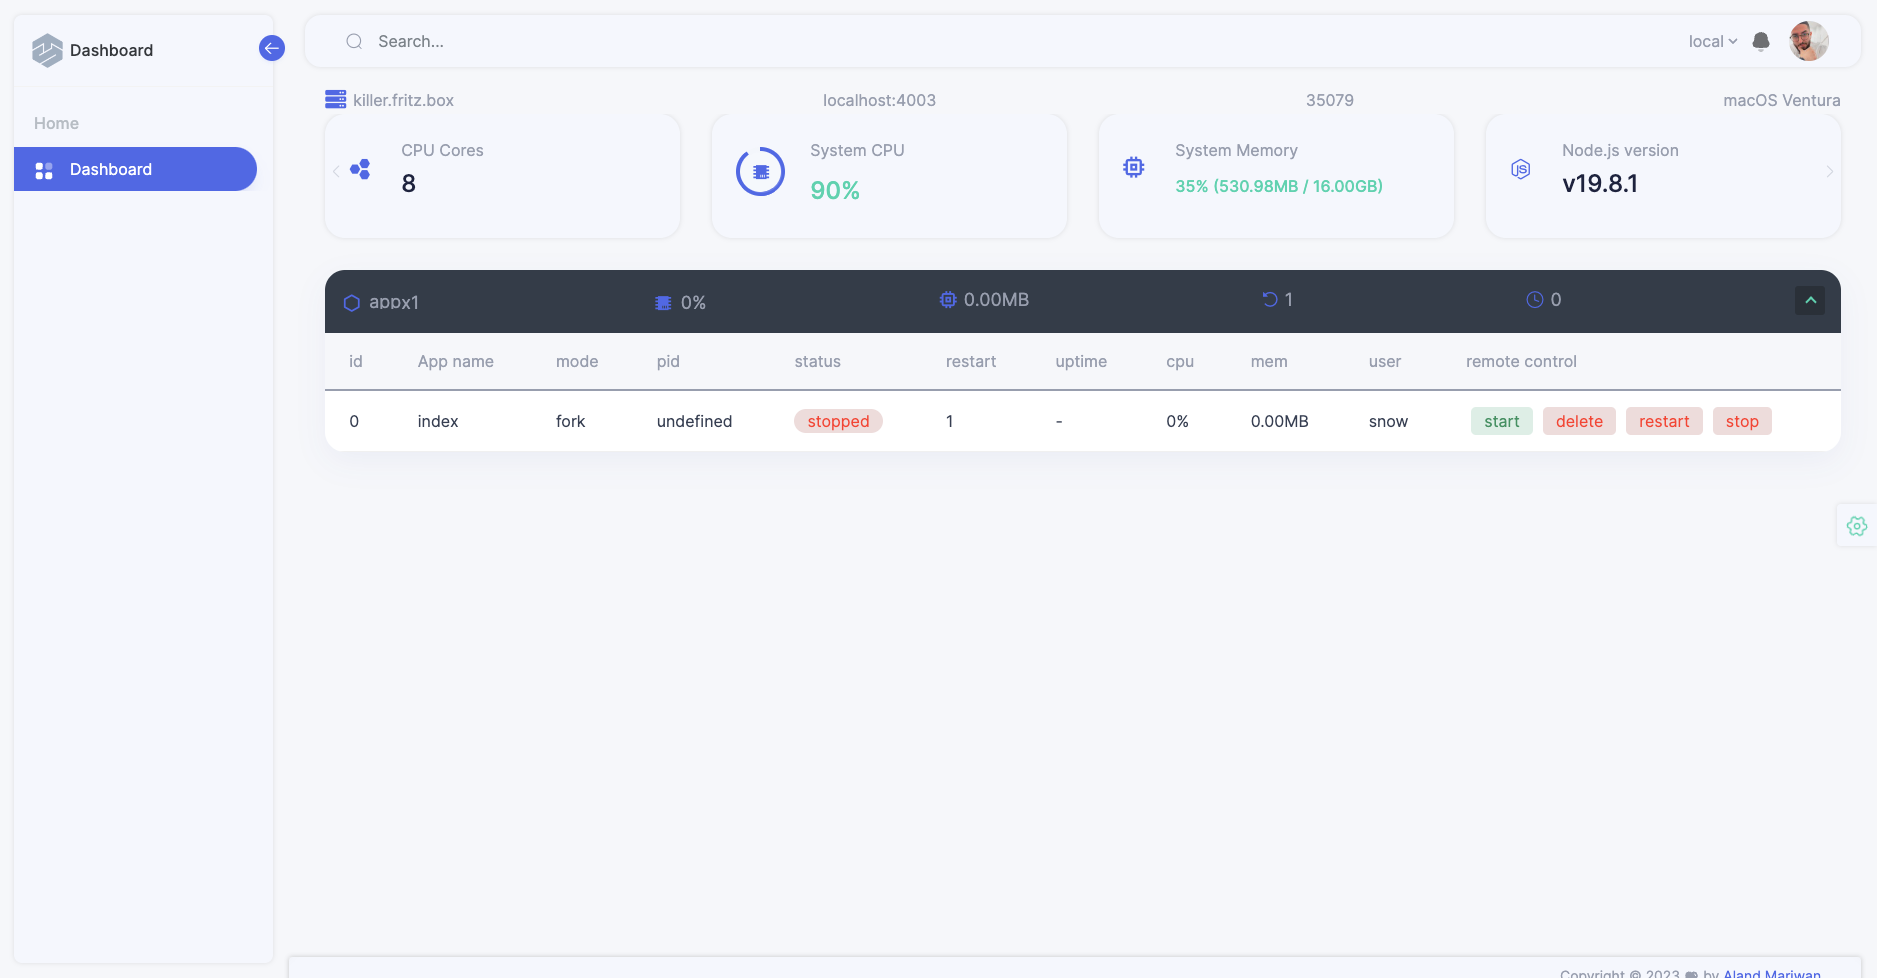
\includegraphics[width=1\textwidth]{img/dashboard.png}
	\caption{Dashboard (Frontend)}
	\label{fig:example}
	\label{Login-Seite}
\end{figure}
	\par\newpage
